\documentclass[aspectratio=169,10pt]{beamer}

\usetheme{default}
\usecolortheme{default}
\setbeamertemplate{navigation symbols}{}
\setbeamertemplate{footline}{}
\setbeamertemplate{frametitle continuation}{}

\usepackage{fontspec}
\usepackage{xeCJK}
\setCJKmainfont{Noto Serif CJK JP}
\setCJKsansfont{Noto Sans CJK JP}
\setCJKmonofont{Noto Sans Mono CJK JP}
\usepackage{microtype}
\usepackage{tikz}
\usepackage{fontawesome5}
\usepackage{graphicx}
\usepackage{hyperref}
\usepackage{calc}
\graphicspath{{logos/}}

\usetikzlibrary{arrows.meta,positioning,shapes.geometric,shapes.misc,fit,backgrounds,calc,decorations.pathreplacing}

% ── Colors ───────────────────────────────────────────────────────────
\definecolor{primary}{HTML}{0891B2}
\definecolor{primarydark}{HTML}{0E7490}
\definecolor{primarylight}{HTML}{67E8F9}
\definecolor{dark}{HTML}{0F172A}
\definecolor{darkcard}{HTML}{1E293B}
\definecolor{text}{HTML}{1E293B}
\definecolor{muted}{HTML}{64748B}
\definecolor{bg}{HTML}{F0F4F8}
\definecolor{cardbg}{HTML}{F8FAFC}
\definecolor{border}{HTML}{E2E8F0}
\definecolor{accentgreen}{HTML}{10B981}
\definecolor{accentamber}{HTML}{F59E0B}
\definecolor{accentred}{HTML}{EF4444}
\definecolor{accentpurple}{HTML}{8B5CF6}
\definecolor{lightcyan}{HTML}{ECFEFF}
\definecolor{lightgreen}{HTML}{ECFDF5}
\definecolor{lightamber}{HTML}{FFFBEB}
\definecolor{lightred}{HTML}{FEF2F2}
\definecolor{lightpurple}{HTML}{F5F3FF}

% ── Beamer Styling ───────────────────────────────────────────────────
\setbeamercolor{background canvas}{bg=bg}
\setbeamercolor{normal text}{fg=text}
\setbeamercolor{frametitle}{fg=text}
\setbeamercolor{item}{fg=primary}

\setbeamerfont{frametitle}{size=\Large,series=\bfseries}
\setbeamerfont{framesubtitle}{size=\small,series=\normalfont}

\setbeamertemplate{frametitle}{
  \vspace{6pt}
  \insertframetitle\par
  \vspace{2pt}
  \textcolor{primary}{\rule{40pt}{2.5pt}}
  \ifx\insertframesubtitle\empty\else
    \par\vspace{2pt}
    {\usebeamerfont{framesubtitle}\color{muted}\insertframesubtitle}
  \fi
  \vspace{4pt}
}

\setbeamertemplate{footline}{
  \hbox to \paperwidth{
    \hspace{16pt}{\color{muted}\tiny OJTFlow}
    \hfill
    {\color{muted}\tiny\insertframenumber}
    \hspace{16pt}
  }\vspace{6pt}
}

% ── Helpers ──────────────────────────────────────────────────────────
\newcommand{\tech}[1]{%
  \tikz[baseline=(t.base)]{\node[fill=lightcyan, rounded corners=3pt, inner xsep=4pt, inner ysep=1.5pt] (t)
    {\scriptsize\bfseries\color{primarydark}#1};}~%
}
\newcommand{\taggreen}[1]{%
  \tikz[baseline=(t.base)]{\node[fill=lightgreen, rounded corners=3pt, inner xsep=4pt, inner ysep=1.5pt] (t)
    {\scriptsize\bfseries\color{accentgreen!80!black}#1};}~%
}
\newcommand{\metric}[2]{%
  \begin{tikzpicture}
    \node[fill=cardbg, draw=border, rounded corners=5pt, inner sep=8pt,
          minimum width=2.4cm, align=center] {
      {\Large\bfseries\color{primary}#1}\par\vspace{1pt}
      {\tiny\color{muted}#2}
    };
  \end{tikzpicture}%
}

\begin{document}

% ═══════════════════════════════════════════════════════════════════════
% SLIDE 1: Title
% ═══════════════════════════════════════════════════════════════════════
{
\setbeamercolor{background canvas}{bg=dark}
\begin{frame}[plain]
  \vfill
  \begin{tikzpicture}[remember picture,overlay]
    \node[fill=primary, rounded corners=8pt, minimum size=36pt,
          anchor=north east] at ([xshift=-24pt,yshift=-20pt]current page.north east)
      {\large\bfseries\color{white}OJT};
  \end{tikzpicture}
  \begin{center}
    {\LARGE\bfseries\color{white}OJTFlow}\\[10pt]
    {\normalsize\color{muted}AI駆動の医療データガバナンス運用システム}\\[3pt]
    {\small\color{primary}基盤モデル\quad\textbar\quad RAG\quad\textbar\quad 永続KG\quad\textbar\quad MCP\quad\textbar\quad マルチエージェント}\\[24pt]
    {\small\color{white}メンバー: Nguyen Tran Nhat Trung}\\[4pt]
    {\small\color{muted}HuReDee-IoYou AI OJTプログラム\quad|\quad 2026年6月}
  \end{center}
  \vfill
\end{frame}
}

% ═══════════════════════════════════════════════════════════════════════
% SLIDE 2: Why OJTFlow (visual comparison)
% ═══════════════════════════════════════════════════════════════════════
\begin{frame}{なぜOJTFlowか？}
\vspace{-4pt}
\centering
\begin{tikzpicture}[
  pain/.style={fill=lightred, draw=accentred!30, rounded corners=6pt,
               minimum width=5.2cm, minimum height=0.7cm, align=left,
               font=\scriptsize, inner xsep=8pt, inner ysep=5pt},
  fix/.style={fill=lightgreen, draw=accentgreen!30, rounded corners=6pt,
              minimum width=5.2cm, minimum height=0.7cm, align=left,
              font=\scriptsize, inner xsep=8pt, inner ysep=5pt},
  hdr/.style={font=\small\bfseries, anchor=south},
  arw/.style={-{Stealth[length=6pt,width=5pt]}, primary, line width=1.5pt}
]
  \node[hdr, color=accentred] at (-3.5,3.1) {現状};
  \node[hdr, color=accentgreen] at (3.5,3.1) {OJTFlowで解決};

  \node[pain] (p1) at (-3.5, 2.4) {\color{accentred}\faTimesCircle\quad \color{text}手動変換でエラー多発};
  \node[pain] (p2) at (-3.5, 1.4) {\color{accentred}\faTimesCircle\quad \color{text}LLMのハルシネーション};
  \node[pain] (p3) at (-3.5, 0.4) {\color{accentred}\faTimesCircle\quad \color{text}監査証跡・承認なし};
  \node[pain] (p4) at (-3.5,-0.6) {\color{accentred}\faTimesCircle\quad \color{text}PHI漏洩リスク};
  \node[pain] (p5) at (-3.5,-1.6) {\color{accentred}\faTimesCircle\quad \color{text}スキーマドリフト未検知};

  \node[fix] (f1) at (3.5, 2.4) {\color{accentgreen}\faCheckCircle\quad \color{text}AI＋ルールベース実行};
  \node[fix] (f2) at (3.5, 1.4) {\color{accentgreen}\faCheckCircle\quad \color{text}RAG根拠付き検証済み出力};
  \node[fix] (f3) at (3.5, 0.4) {\color{accentgreen}\faCheckCircle\quad \color{text}完全な監査＋人間レビュー};
  \node[fix] (f4) at (3.5,-0.6) {\color{accentgreen}\faCheckCircle\quad \color{text}PHI自動検出・墨消し};
  \node[fix] (f5) at (3.5,-1.6) {\color{accentgreen}\faCheckCircle\quad \color{text}スキーマレジストリ＋通知};

  \foreach \i in {1,...,5} {
    \draw[arw] (p\i.east) -- (f\i.west);
  }

  \node[fill=lightcyan, draw=primary!20, rounded corners=5pt,
        minimum width=12cm, minimum height=0.8cm, align=center,
        font=\scriptsize\bfseries\color{primarydark}] at (0,-2.8)
    {5エージェント\quad\textbar\quad 35+ エンドポイント\quad\textbar\quad 6 MCPサーバー\quad\textbar\quad MarkItDown/MinerU\quad\textbar\quad 永続知識グラフ};
\end{tikzpicture}
\end{frame}

% ═══════════════════════════════════════════════════════════════════════
% SLIDE 4: LLM + MCP Runtime Flow
% ═══════════════════════════════════════════════════════════════════════
\begin{frame}{LLM + MCP 実行フロー}
\vspace{-6pt}
\centering
\begin{tikzpicture}[
  flow/.style={fill=cardbg, draw=border, rounded corners=5pt,
               minimum width=2.15cm, minimum height=0.9cm,
               text width=1.9cm, align=center, font=\tiny, inner sep=4pt},
  wide/.style={fill=cardbg, draw=border, rounded corners=6pt,
               minimum width=5.65cm, minimum height=1.05cm,
               text width=5.2cm, align=left, font=\tiny, inner sep=7pt},
  timeline/.style={fill=lightgreen, draw=accentgreen!20, rounded corners=5pt,
                   minimum width=11.8cm, minimum height=0.75cm,
                   text width=11.3cm, align=center, font=\tiny, inner sep=5pt},
  arr/.style={-{Stealth[length=3pt,width=3pt]}, primary!70, line width=0.8pt},
  thinarr/.style={-{Stealth[length=2pt,width=2pt]}, muted!45, line width=0.35pt}
]
  \path[use as bounding box] (-6.15,-3.05) rectangle (6.15,2.35);

  \node[flow, fill=lightcyan, draw=primary!25] (ui) at (-4.9,1.65)
    {{\bfseries\color{primarydark}UI stream}\\{\color{muted}\texttt{/assistant/chat}}\\{\color{muted}\texttt{/stream}}};
  \node[flow] (ctx) at (-2.45,1.65)
    {{\bfseries\color{text}Context}\\{\color{muted}session}\\{\color{muted}memory, files}};
  \node[flow, fill=lightpurple, draw=accentpurple!25] (planner) at (0,1.65)
    {{\bfseries\color{accentpurple}Planner LLM}\\{\color{muted}設定モデル}\\{\color{muted}gpt-5-mini}};
  \node[flow, fill=lightamber, draw=accentamber!30] (schema) at (2.45,1.65)
    {{\bfseries\color{accentamber!80!black}JSON plan}\\{\color{muted}tool names}\\{\color{muted}arguments}};
  \node[flow, fill=lightgreen, draw=accentgreen!25] (catalog) at (4.9,1.65)
    {{\bfseries\color{accentgreen!80!black}MCP catalog}\\{\color{muted}12 tools}\\{\color{muted}max 4 calls}};

  \draw[arr] (ui) -- (ctx);
  \draw[arr] (ctx) -- (planner);
  \draw[arr] (planner) -- (schema);
  \draw[arr] (schema) -- (catalog);

  \node[wide, fill=lightgreen, draw=accentgreen!25] (exec) at (-3.05,0.15) {
    {\color{accentgreen}\faServer\quad \scriptsize\bfseries\color{text}Backend / MCP executor}\\[2pt]
    {\color{muted}retrieval、validation、workflow、reviewのみallowlist実行。}\\[1pt]
    {\color{muted}\texttt{/assistant/tools}, \texttt{/assistant/mcp/resources}, \texttt{/assistant/mcp/prompts}}
  };
  \node[wide, fill=lightred, draw=accentred!20] (guard) at (3.05,0.15) {
    {\color{accentred}\faLock\quad \scriptsize\bfseries\color{text}Governed execution}\\[2pt]
    {\color{muted}prompt-injection boundary、plan validation、cost/provider policy。}\\[1pt]
    {\color{muted}Write actionは明示確認までゲート。}
  };

  \draw[arr] (schema.south) -- ([yshift=3pt]exec.north);
  \draw[arr] (catalog.south) -- ([yshift=3pt]guard.north);
  \draw[arr] (exec) -- (guard);

  \node[flow, minimum width=2.4cm, text width=2.15cm] (audit) at (-3.7,-1.25)
    {{\bfseries\color{text}Audit + replay}\\{\color{muted}tool audit}\\{\color{muted}stream events}};
  \node[flow, fill=lightpurple, draw=accentpurple!25, minimum width=2.4cm, text width=2.15cm] (synth) at (0,-1.25)
    {{\bfseries\color{accentpurple}Synthesis LLM}\\{\color{muted}tool結果}\\{\color{muted}から回答}};
  \node[flow, fill=lightcyan, draw=primary!20, minimum width=2.4cm, text width=2.15cm] (answer) at (3.7,-1.25)
    {{\bfseries\color{primarydark}Answer stream}\\{\color{muted}\texttt{answer\_delta}}\\{\color{muted}\texttt{final}}};

  \draw[arr] (exec.south) -- (audit.north);
  \draw[arr] (guard.south) -- (synth.north);
  \draw[arr] (synth) -- (answer);

  \node[timeline] at (0,-2.55) {
    {\color{accentgreen}\faClipboard\quad \bfseries\color{text}Live timeline:\quad}
    {\color{muted}\texttt{stream\_opened} $\rightarrow$ \texttt{planning\_started} $\rightarrow$ \texttt{plan\_ready} $\rightarrow$ \texttt{tool\_started/completed} $\rightarrow$ \texttt{synthesis\_started} $\rightarrow$ \texttt{answer\_delta} $\rightarrow$ \texttt{final}}
  };
\end{tikzpicture}
\end{frame}

% ═══════════════════════════════════════════════════════════════════════
% SLIDE 5: Architecture (full-width diagram)
% ═══════════════════════════════════════════════════════════════════════
\begin{frame}{システムアーキテクチャ}
\vspace{-6pt}
\centering
\begin{tikzpicture}[
  layer/.style={rounded corners=6pt, minimum height=1cm, align=center,
                font=\scriptsize, inner sep=6pt},
  comp/.style={fill=cardbg, draw=border, rounded corners=4pt,
               minimum height=0.55cm, font=\tiny, inner xsep=5pt},
  arr/.style={-{Stealth[length=5pt]}, primary!60, thick},
  lbl/.style={font=\tiny\bfseries, color=primary}
]
  \node[layer, fill=lightcyan, draw=primary!25, minimum width=13cm] (ul) at (0,2.8) {};
  \node[lbl, anchor=west] at ([xshift=6pt]ul.west) {ユーザー};
  \node[comp] at (-3, 2.8) {
\includegraphics[height=8pt]{react.png}~React 18 + Radix UI};
  \node[comp] at (0.2, 2.8) {
\includegraphics[height=8pt]{typescript.png}~TypeScript};
  \node[comp] at (2.4, 2.8) {AIチャット};
  \node[comp] at (4.6, 2.8) {MCPクライアント};

  \node[layer, fill=primary!8, draw=primary!20, minimum width=13cm] (ol) at (0,1.4) {};
  \node[lbl, anchor=west] at ([xshift=6pt]ol.west) {制御};
  \node[comp] at (-3, 1.4) {
\includegraphics[height=8pt]{fastapi.png}~FastAPI};
  \node[comp] at (-0.8, 1.4) {
\includegraphics[height=8pt]{python.png}~ワークフロー};
  \node[comp] at (1.8, 1.4) {レビューゲート};
  \node[comp] at (4, 1.4) {MarkItDown / MinerU};

  \node[layer, fill=accentgreen!6, draw=accentgreen!20, minimum width=13cm] (cl) at (0,0) {};
  \node[lbl, anchor=west, color=accentgreen!70!black] at ([xshift=6pt]cl.west) {コア};
  \node[comp] at (-2.8, 0) {コントラクト};
  \node[comp] at (-0.6, 0) {ポリシー};
  \node[comp] at (1.6, 0) {データツール};
  \node[comp] at (4, 0) {5エージェント};

  \node[layer, fill=accentamber!6, draw=accentamber!20, minimum width=13cm] (il) at (0,-1.4) {};
  \node[lbl, anchor=west, color=accentamber!70!black] at ([xshift=6pt]il.west) {基盤};
  \node[comp] at (-3.2,-1.4) {
\includegraphics[height=8pt]{postgresql.png}~PostgreSQL};
  \node[comp] at (-0.4,-1.4) {
\includegraphics[height=8pt]{keycloak.png}~Keycloak};
  \node[comp] at (1.6,-1.4) {
\includegraphics[height=8pt]{minio.png}~MinIO};
  \node[comp] at (3.4,-1.4) {
\includegraphics[height=8pt]{redis.png}~Redis};
  \node[comp] at (5.2,-1.4) {
\includegraphics[height=8pt]{docker.png}~Docker};

  \draw[arr] ([yshift=-2pt]ul.south) -- ([yshift=2pt]ol.north);
  \draw[arr] ([yshift=-2pt]ol.south) -- ([yshift=2pt]cl.north);
  \draw[arr] ([yshift=-2pt]cl.south) -- ([yshift=2pt]il.north);

\end{tikzpicture}
\end{frame}

% ═══════════════════════════════════════════════════════════════════════
% SLIDE 6: Docker Internal Network
% ═══════════════════════════════════════════════════════════════════════
\begin{frame}{Docker内部ネットワーク}
\vspace{-6pt}
\centering
\begin{tikzpicture}[
  svc/.style={fill=cardbg, draw=border, rounded corners=5pt,
              minimum width=1.55cm, minimum height=0.62cm,
              text width=1.32cm, align=center, font=\tiny, inner sep=3pt},
  ext/.style={fill=lightamber, draw=accentamber!35, rounded corners=5pt,
              minimum width=1.75cm, minimum height=0.58cm,
              text width=1.45cm, align=center, font=\tiny, inner sep=3pt},
  arr/.style={-{Stealth[length=3pt,width=3pt]}, primary!70, line width=0.8pt},
  thinarr/.style={-{Stealth[length=2pt,width=2pt]}, draw=muted!45, line width=0.35pt}
]
  \path[use as bounding box] (-6.25,-3.0) rectangle (6.25,2.75);

  \node[svc, fill=lightcyan, draw=primary!30] (browser) at (-5.25,1.25)
    {{\color{primarydark}\faGlobe}\\[-1pt]{\bfseries Browser}\\{\color{muted}\texttt{:15173}}};
  \node[svc, fill=lightcyan, draw=primary!25] (fe) at (-3.25,1.25)
    {
\includegraphics[height=7pt]{nginx.png}\\[-1pt]{\bfseries frontend}\\{\color{muted}nginx \texttt{:5173}}};
  \node[svc, fill=lightgreen, draw=accentgreen!25] (api) at (-1.25,1.25)
    {
\includegraphics[height=7pt]{fastapi.png}\\[-1pt]{\bfseries API}\\{\color{muted}\texttt{api:8000}}};

  \node[svc] (kc) at (1.25,2.12)
    {
\includegraphics[height=7pt]{keycloak.png}\\[-1pt]Keycloak\\{\color{muted}\texttt{:8080}}};
  \node[svc] (pg) at (3.05,2.12)
    {
\includegraphics[height=7pt]{postgresql.png}\\[-1pt]Postgres\\{\color{muted}\texttt{:5432}}};
  \node[svc] (redis) at (4.85,2.12)
    {
\includegraphics[height=7pt]{redis.png}\\[-1pt]Redis\\{\color{muted}\texttt{:6379}}};
  \node[svc] (mq) at (1.25,1.1)
    {
\includegraphics[height=7pt]{rabbitmq.png}\\[-1pt]RabbitMQ\\{\color{muted}\texttt{:5672}}};
  \node[svc] (minio) at (3.05,1.1)
    {
\includegraphics[height=7pt]{minio.png}\\[-1pt]MinIO\\{\color{muted}\texttt{:9000}}};
  \node[svc] (gms) at (4.85,1.1)
    {graph-med\\service\\{\color{muted}\texttt{:8010}}};
  \node[svc, fill=lightgreen, draw=accentgreen!25] (medsig) at (1.25,0.08)
    {MedSigLIP\\API\\{\color{muted}\texttt{:8000}}};
  \node[svc, fill=lightpurple, draw=accentpurple!25] (workers) at (3.05,0.08)
    {
\includegraphics[height=7pt]{celery-light.png}\\[-1pt]Celery\\workers};
  \node[svc, fill=lightpurple, draw=accentpurple!25] (models) at (4.85,0.08)
    {graph-med\\LLM / embed\\{\color{muted}\texttt{:8000}}};
  \node[ext] (neo4j) at (4.85,-0.98)
    {external\\Neo4j\\{\color{muted}\texttt{:7688}}};

  \begin{scope}[on background layer]
    \node[fill=white, draw=border, rounded corners=7pt,
          fit=(kc)(pg)(redis)(mq)(minio)(gms)(medsig)(workers)(models),
          inner xsep=8pt, inner ysep=12pt] (services) {};
    \node[fill=white, draw=primary!25, rounded corners=8pt,
          fit=(fe)(api)(services),
          inner xsep=14pt, inner ysep=14pt] (dockerbox) {};
    \node[fill=primary!4, draw=primary!25, dashed, rounded corners=7pt,
          fit=(api)(services),
          inner xsep=10pt, inner ysep=10pt] (backendbox) {};
  \end{scope}

  \node[anchor=north west, font=\tiny\bfseries, color=primarydark]
    at ([xshift=6pt,yshift=-4pt]dockerbox.north west) {Docker Compose内部ネットワーク};
  \node[anchor=north west, font=\tiny\bfseries, color=primarydark]
    at ([xshift=8pt,yshift=-15pt]backendbox.north west) {プライベート・バックエンド層};
  \node[anchor=north west, font=\tiny\bfseries, color=text]
    at ([xshift=8pt,yshift=-5pt]services.north west) {Docker DNS経由のバックエンドサービス};

  \draw[arr] (browser) -- node[above, font=\tiny, color=muted]{公開host port} (fe);
  \draw[arr] (fe) -- node[above, font=\tiny, color=muted]{Docker DNS \texttt{api:8000}} (api);
  \foreach \target in {kc,pg,redis,mq,minio,gms,medsig} {
    \draw[thinarr] (api) -- (\target);
  }
  \draw[thinarr] (mq) -- (workers);
  \draw[thinarr] (workers) -- (pg);
  \draw[thinarr] (workers) -- (minio);
  \draw[thinarr] (gms) -- (models);
  \draw[thinarr, draw=accentamber!75!black] (gms) -- node[right, font=\tiny, color=muted]{Bolt} (neo4j);

  \node[fill=lightcyan, draw=primary!20, rounded corners=5pt,
        minimum width=11.7cm, minimum height=0.55cm, align=center,
        font=\tiny\bfseries\color{primarydark}] at (0,-2.35)
    {公開するのはブラウザ向けポートのみ。バックエンド間通信はDocker DNS内で完結。クラウドではHTTPS ingress + private VPCへ置換。};
\end{tikzpicture}
\end{frame}

% ═══════════════════════════════════════════════════════════════════════
% SLIDE 7: Multi-Agent System (hub diagram)
% ═══════════════════════════════════════════════════════════════════════
\begin{frame}{マルチエージェントシステム}
\vspace{-2pt}
\centering
\begin{tikzpicture}[
  agent/.style={fill=cardbg, draw=border, rounded corners=6pt,
                minimum width=2.6cm, minimum height=1.1cm, align=center,
                font=\scriptsize, inner sep=4pt},
  hub/.style={fill=primary, rounded corners=10pt, minimum size=2.2cm,
              align=center, font=\small\bfseries, text=white},
  conn/.style={primary!40, thick, -{Stealth[length=4pt]}}
]
  \node[hub] (h) at (0,0) {オーケストレータ\\{\tiny\color{white!80}共有状態}};

  \node[agent, fill=lightcyan] (a1) at (-5, 1.5) {\bfseries\color{primarydark}パーサー\\{\tiny\color{muted}CSV / JSON / YAML}};
  \node[agent, fill=lightcyan] (a2) at (-5,-1.5) {\bfseries\color{primarydark}バリデーター\\{\tiny\color{muted}スキーマ検証}};
  \node[agent, fill=lightgreen] (a3) at (5, 1.5) {\bfseries\color{accentgreen!80!black}トランスフォーマー\\{\tiny\color{muted}フォーマット変換}};
  \node[agent, fill=lightamber] (a4) at (5,-1.5) {\bfseries\color{accentamber!80!black}セーフティ\\{\tiny\color{muted}PHI / 脅威スキャン}};
  \node[agent, fill=lightpurple] (a5) at (0,-3) {\bfseries\color{accentpurple!80!black}エクスプレイナー\\{\tiny\color{muted}監査レポート}};

  \draw[conn] (a1.east) -- (h); \draw[conn] (a2.east) -- (h);
  \draw[conn] (h) -- (a3.west); \draw[conn] (h) -- (a4.west);
  \draw[conn] (h) -- (a5.north);

  \node[fill=accentgreen!15, rounded corners=3pt, font=\tiny\bfseries,
        color=accentgreen!80!black, inner xsep=5pt, inner ysep=2pt]
    at (0, 2.2) {ルールベース --- データ操作にLLM推測なし};
\end{tikzpicture}
\end{frame}

% ═══════════════════════════════════════════════════════════════════════
% SLIDE 6: RAG Pipeline (flow diagram)
% ═══════════════════════════════════════════════════════════════════════
\begin{frame}{RAG検索パイプライン}
\vspace{-2pt}
\centering
\begin{tikzpicture}[
  box/.style={fill=cardbg, draw=border, rounded corners=5pt,
              minimum width=2.2cm, minimum height=1.6cm, align=center,
              font=\tiny, inner sep=4pt},
  rag arrow/.style={-{Stealth[length=5pt]}, primary, thick}
]
  \node[box] (q) at (0,0) {{\tiny\bfseries\color{primarydark}クエリ}\\[2pt]{\tiny\color{muted}自然言語}};
  \node[box] (e) at (2.8,0) {{\tiny\bfseries\color{primarydark}埋め込み}\\[2pt]{\tiny\color{muted}384d vectors}};
  \node[box] (v) at (5.6,0) {{\tiny\bfseries\color{primarydark}ベクトル検索}\\[2pt]{\tiny\color{muted}pgvector}};
  \node[box] (m) at (8.4,0) {{\tiny\bfseries\color{primarydark}ソースMMR}\\[2pt]{\tiny\color{muted}多様性}};
  \node[box] (r) at (11.2,0) {{\tiny\bfseries\color{primarydark}リランク}\\[2pt]{\tiny\color{muted}CrossEncoder}};

  \draw[rag arrow] (q) -- (e);
  \draw[rag arrow] (e) -- (v);
  \draw[rag arrow] (v) -- (m);
  \draw[rag arrow] (m) -- (r);

  \node[fill=lightcyan, draw=border, rounded corners=5pt,
        minimum width=12.5cm, minimum height=0.8cm, align=center,
        font=\tiny, inner sep=6pt] (kb) at (5.6,-2)
    {\bfseries\color{primarydark}知識ベース:\quad
     \color{muted}スキーマ~~|~~FHIR~~|~~ガバナンス~~|~~臨床用語~~|~~データ辞書};

  \draw[primary, thick, dashed, -{Stealth[length=4pt]}] (kb) -- (v);

  \node[fill=lightgreen, draw=border, rounded corners=5pt,
        minimum width=2.2cm, minimum height=0.8cm, align=center,
        font=\tiny, inner sep=4pt] at (11.2,-2)
    {\bfseries\color{accentgreen}品質管理\\\color{muted}鮮度 | 整合性};

  \node[fill=lightpurple, draw=border, rounded corners=5pt,
        minimum width=4.2cm, minimum height=0.6cm, align=center,
        font=\tiny, inner sep=4pt] (gh) at (9.8, 1.6)
    {\bfseries\color{accentpurple}永続KG\quad
     \color{muted}Neo4j / Kuzu};
  \draw[accentpurple, thick, -{Stealth[length=4pt]}] (r) -- (gh);
\end{tikzpicture}
\end{frame}

% ═══════════════════════════════════════════════════════════════════════
% SLIDE 7: MedSigLIP Contrastive Pretraining
% ═══════════════════════════════════════════════════════════════════════
\begin{frame}{MedSigLIP Pretrain: ENTRep + Contrastive Learning}
\vspace{-5pt}
\centering
\begin{tikzpicture}[
  card/.style={fill=cardbg, draw=border, rounded corners=6pt,
               minimum width=3.45cm, minimum height=1.45cm,
               text width=3.05cm, align=center, font=\tiny, inner sep=6pt},
  arr/.style={-{Stealth[length=5pt]}, primary, thick}
]
  \node[card, fill=lightcyan, draw=primary!25] (entrep) at (-4.15,0.9)
    {{\scriptsize\bfseries\color{primarydark}ENTRep Challenge}\\[2pt]
     {\color{muted}ACM MM 2025}\\
     {\color{muted}ENT endoscopy images}};

  \node[card, fill=lightgreen, draw=accentgreen!25] (pairs) at (0,0.9)
    {{\scriptsize\bfseries\color{accentgreen!80!black}Image-text pairs}\\[2pt]
     {\color{muted}ENT画像 + label}\\
     {\color{muted}clinical text prompt}\\
     {\color{muted}retrieval supervision}};

  \node[card, fill=lightpurple, draw=accentpurple!25] (pretrain) at (4.15,0.9)
    {{\scriptsize\bfseries\color{accentpurple}Contrastive pretrain}\\[2pt]
     {\color{muted}image encoder}\\
     {\color{muted}text encoder}\\
     {\color{muted}shared embedding space}};

  \draw[arr] (entrep) -- (pairs);
  \draw[arr] (pairs) -- (pretrain);

  \node[fill=white, draw=border, rounded corners=6pt,
        minimum width=11.9cm, minimum height=0.95cm,
        text width=11.3cm, align=center, font=\scriptsize, inner sep=7pt] at (0,-1.0)
    {{\bfseries\color{text}OJTFlowでの利用:}
     {\color{muted} ENTRepでOJTFlow MedSigLIPをadapt。正しいimage-text pairを近づけ、誤ったpairを離す。画像分類、text-to-image search、similar-image retrievalに利用。}};

  \node[fill=lightamber, draw=accentamber!25, rounded corners=5pt,
        minimum width=11.9cm, minimum height=0.55cm,
        text width=11.3cm, align=center, font=\tiny, inner sep=5pt] at (0,-2.25)
    {{\bfseries\color{accentamber!80!black}Source:}
     \href{https://aichallenge.hcmus.edu.vn/acm-mm-2025/entrep}{\color{primarydark}aichallenge.hcmus.edu.vn/acm-mm-2025/entrep}};
\end{tikzpicture}
\end{frame}

% ═══════════════════════════════════════════════════════════════════════
% SLIDE 7: Persistent Corpus Knowledge Graph
% ═══════════════════════════════════════════════════════════════════════
\begin{frame}{永続コーパス知識グラフ}
\vspace{-6pt}
\centering
\begin{tikzpicture}[
  box/.style={fill=cardbg, draw=border, rounded corners=6pt,
              minimum width=2.55cm, minimum height=1.15cm, align=center,
              font=\tiny, inner sep=5pt},
  store/.style={fill=lightpurple, draw=accentpurple!25, rounded corners=6pt,
                minimum width=2.8cm, minimum height=1.25cm, align=center,
                font=\tiny, inner sep=5pt},
  card/.style={fill=cardbg, draw=border, rounded corners=5pt,
               minimum width=5.5cm, minimum height=1.05cm,
               text width=5.05cm, align=left, font=\tiny, inner sep=6pt},
  arr/.style={-{Stealth[length=5pt]}, primary, thick}
]
  \node[box] (c) at (-4.4, 1.55) {{\bfseries\color{primarydark}コーパスチャンク}\\{\color{muted}PDF, FHIR, CSV, notes}};
  \node[box] (r) at (-1.45, 1.55) {{\bfseries\color{primarydark}コード辞書}\\{\color{muted}\texttt{medical\_concepts.json}}};
  \node[store] (kg) at (1.55, 1.55) {{\bfseries\color{accentpurple}KGリポジトリ}\\{\color{muted}Neo4j標準}\\{\color{muted}Kuzu / memory adapters}};
  \node[box] (ui) at (4.55, 1.55) {{\bfseries\color{primarydark}/knowledge UI}\\{\color{muted}Graph + Search tabs}};

  \draw[arr] (c) -- (r);
  \draw[arr] (r) -- (kg);
  \draw[arr] (kg) -- (ui);

  \node[card] at (-2.95, -0.05) {
    {\color{primary}\faCheckCircle\quad \scriptsize\bfseries\color{text}決定的インポート}\\[2pt]
    {\tiny\color{muted}別名、表示名、信頼コードを照合し、未解決の自由文はグラフノード化しない。}
  };
  \node[card] at (2.95, -0.05) {
    {\color{accentpurple}\faSearch\quad \scriptsize\bfseries\color{text}グラフ探索API}\\[2pt]
    {\tiny\color{muted}\texttt{/search}, \texttt{/neighborhood}, \texttt{/nodes/\{id\}}, \texttt{/stats}, \texttt{/import}を\texttt{/api/v1/knowledge-graph}で提供。}
  };
  \node[card] at (-2.95, -1.45) {
    {\color{accentgreen}\faLock\quad \scriptsize\bfseries\color{text}ワークスペーススコープ}\\[2pt]
    {\tiny\color{muted}読み取りはglobal概念と呼び出し元組織を統合し、書き込みは組織の由来を保持。}
  };
  \node[card] at (2.95, -1.45) {
    {\color{accentamber}\faClipboard\quad \scriptsize\bfseries\color{text}エビデンス由来}\\[2pt]
    {\tiny\color{muted}ノードとエッジにchunk ID、source snippet、confidence、review stateを保持。}
  };

  \node[fill=lightcyan, draw=primary!20, rounded corners=5pt,
        minimum width=11.8cm, minimum height=0.6cm, align=center,
        font=\tiny\bfseries\color{primarydark}] at (0,-2.85)
    {graph-med互換Neo4j ontology + OJT source-backed overlay};
\end{tikzpicture}
\end{frame}

% ═══════════════════════════════════════════════════════════════════════
% SLIDE 8: Data Flow (end-to-end pipeline)
% ═══════════════════════════════════════════════════════════════════════
\begin{frame}{エンドツーエンドのデータフロー}
\vspace{-4pt}
\centering
\begin{tikzpicture}[
  stp/.style={rounded corners=6pt, minimum width=1.7cm, minimum height=2.4cm,
              align=center, font=\tiny, inner sep=4pt},
  arr/.style={-{Stealth[length=5pt,width=4pt]}, thick},
  circ/.style={circle, minimum size=0.7cm, inner sep=0pt}
]
  \node[stp, fill=lightcyan, draw=primary!25] (s1) at (0,0) {};
  \node[circ, fill=primary] at ([yshift=6pt]s1.center) {\normalsize\color{white}\faUpload};
  \node[font=\tiny\bfseries, color=primarydark] at ([yshift=-12pt]s1.center) {アップロード};
  \node[font=\tiny, color=muted] at ([yshift=-20pt]s1.center) {CSV/JSON};

  \node[stp, fill=lightcyan, draw=primary!25] (s2) at (2.3,0) {};
  \node[circ, fill=primary] at ([yshift=6pt]s2.center) {\normalsize\color{white}\faCogs};
  \node[font=\tiny\bfseries, color=primarydark] at ([yshift=-12pt]s2.center) {解析};
  \node[font=\tiny, color=muted] at ([yshift=-20pt]s2.center) {プロファイル};

  \node[stp, fill=lightamber, draw=accentamber!25] (s3) at (4.6,0) {};
  \node[circ, fill=accentamber] at ([yshift=6pt]s3.center) {\normalsize\color{white}\faClipboard};
  \node[font=\tiny\bfseries, color=accentamber!80!black] at ([yshift=-12pt]s3.center) {検証};
  \node[font=\tiny, color=muted] at ([yshift=-20pt]s3.center) {スキーマ};

  \node[stp, fill=lightred, draw=accentred!25] (s4) at (6.9,0) {};
  \node[circ, fill=accentred] at ([yshift=6pt]s4.center) {\normalsize\color{white}\faFlag};
  \node[font=\tiny\bfseries, color=accentred!80!black] at ([yshift=-12pt]s4.center) {フラグ};
  \node[font=\tiny, color=muted] at ([yshift=-20pt]s4.center) {課題};

  \node[stp, fill=lightamber, draw=accentamber!25] (s5) at (9.2,0) {};
  \node[circ, fill=accentamber] at ([yshift=6pt]s5.center) {\normalsize\color{white}\faUser};
  \node[font=\tiny\bfseries, color=accentamber!80!black] at ([yshift=-12pt]s5.center) {レビュー};
  \node[font=\tiny, color=muted] at ([yshift=-20pt]s5.center) {人間};

  \node[stp, fill=lightgreen, draw=accentgreen!25] (s6) at (11.5,0) {};
  \node[circ, fill=accentgreen] at ([yshift=6pt]s6.center) {\normalsize\color{white}\faCheck};
  \node[font=\tiny\bfseries, color=accentgreen!80!black] at ([yshift=-12pt]s6.center) {変換};
  \node[font=\tiny, color=muted] at ([yshift=-20pt]s6.center) {JSON};

  \draw[arr, primary!50] (s1) -- (s2); \draw[arr, primary!50] (s2) -- (s3);
  \draw[arr, accentamber!50] (s3) -- (s4); \draw[arr, accentred!50] (s4) -- (s5);
  \draw[arr, accentgreen!50] (s5) -- (s6);

  \node[fill=cardbg, draw=border, rounded corners=5pt,
        minimum width=12.5cm, minimum height=1cm, align=center,
        font=\tiny] (out) at (5.75,-2.4) {
    \bfseries\color{primarydark}出力:\quad
    \color{muted}クリーンJSON\quad+\quad 説明レポート\quad+\quad 監査イベント\quad+\quad エビデンス添付
  };
  \draw[primary, thick, dashed, -{Stealth[length=4pt]}] (s6.south) -- (11.5,-1.9);

  \node[fill=primary!8, rounded corners=3pt, font=\tiny, color=muted,
        inner xsep=6pt, inner ysep=3pt] at (5.75, 2)
    {全ステップを記録 $\rightarrow$ ハッシュチェーン整合性付き追記専用イベントストリーム};
\end{tikzpicture}
\end{frame}

% ═══════════════════════════════════════════════════════════════════════
% SLIDE 9: Security (layered shield + list)
% ═══════════════════════════════════════════════════════════════════════
\begin{frame}{セキュリティとガバナンス}
\vspace{-6pt}
\begin{columns}[T]
  \begin{column}{0.48\textwidth}
    \centering
    \begin{tikzpicture}[
      ring/.style={rounded corners=8pt, draw, thick, align=center, inner sep=6pt}
    ]
      \node[ring, fill=accentred!6, draw=accentred!30,
            minimum width=5.4cm, minimum height=4.8cm] (r1) at (0,0) {};
      \node[font=\tiny\bfseries, color=accentred!70!black, anchor=north]
        at ([yshift=-3pt]r1.north) {OWASP LLM Top 10};

      \node[ring, fill=accentamber!6, draw=accentamber!30,
            minimum width=4.2cm, minimum height=3.4cm] (r2) at (0,-0.2) {};
      \node[font=\tiny\bfseries, color=accentamber!70!black, anchor=north]
        at ([yshift=-3pt]r2.north) {PHI保護};

      \node[ring, fill=accentgreen!6, draw=accentgreen!30,
            minimum width=3cm, minimum height=2cm] (r3) at (0,-0.4) {};
      \node[font=\tiny\bfseries, color=accentgreen!70!black, anchor=north]
        at ([yshift=-3pt]r3.north) {監査証跡};

      \node[fill=primary, rounded corners=5pt, minimum size=0.8cm,
            font=\tiny\bfseries, text=white] at (0,-0.6) {データ};
    \end{tikzpicture}
  \end{column}
  \begin{column}{0.48\textwidth}
    \vspace{6pt}
    \begin{tikzpicture}[
      row/.style={fill=cardbg, draw=border, rounded corners=4pt,
                  minimum width=5.4cm, minimum height=0.7cm,
                  font=\tiny, inner xsep=6pt, align=left}
    ]
      \node[row] (r1) at (0, 0)   {\color{accentred}\faExclamationTriangle\quad \color{text}プロンプトインジェクション防御};
      \node[row] (r2) at (0,-0.9) {\color{accentamber}\faEye\quad \color{text}機密フィールド自動墨消し};
      \node[row] (r3) at (0,-1.8) {\color{accentgreen}\faLink\quad \color{text}ハッシュチェーンイベント整合性};
      \node[row] (r4) at (0,-2.7) {\color{primary}\faLock\quad \color{text}Keycloak SSO + HTTP-Onlyクッキー};
      \node[row] (r5) at (0,-3.6) {\color{primary}\faUser\quad \color{text}リスク操作に人間ゲート};
      \node[row] (r6) at (0,-4.5) {\color{muted}\faServer\quad \color{text}4段階デプロイモード};
    \end{tikzpicture}
  \end{column}
\end{columns}
\end{frame}

% ═══════════════════════════════════════════════════════════════════════
% SLIDE 10: Production Operations
% ═══════════════════════════════════════════════════════════════════════
\begin{frame}{本番運用基盤}
\vspace{-4pt}
\centering
\begin{tikzpicture}[
  card/.style={fill=cardbg, draw=border, rounded corners=6pt,
               minimum width=5.9cm, minimum height=1.35cm,
               align=left, font=\tiny, inner sep=7pt},
  chip/.style={fill=lightcyan, draw=primary!20, rounded corners=4pt,
               font=\tiny\bfseries, inner xsep=5pt, inner ysep=2pt,
               text=primarydark}
]
  \node[card] at (-3.3, 1.75) {
    {
\includegraphics[height=9pt]{rabbitmq.png}~
\includegraphics[height=9pt]{celery.png}\quad \scriptsize\bfseries\color{text}永続バックグラウンドジョブ}\\[3pt]
    {\tiny\color{muted}
\includegraphics[height=6pt]{rabbitmq.png}~RabbitMQ + 
\includegraphics[height=6pt]{celery.png}~CeleryでOCR、RAG、埋め込み、取込、エクスポートを分離}\\[2pt]
    {\tiny\color{muted}\texttt{/api/v1/jobs}で一覧、確認、キャンセル}
  };
  \node[card] at (3.3, 1.75) {
    {
\includegraphics[height=9pt]{prometheus.png}~
\includegraphics[height=9pt]{grafana.png}\quad \scriptsize\bfseries\color{text}可観測性スタック}\\[3pt]
    {\tiny\color{muted}
\includegraphics[height=6pt]{prometheus.png}~Prometheus \texttt{/metrics}、
\includegraphics[height=6pt]{grafana.png}~Grafana、RabbitMQ/Celery exporters}\\[2pt]
    {\tiny\color{muted}Loki + PromtailログとAPI/worker向けSentryフック}
  };
  \node[card] at (-3.3, 0.05) {
    {\color{primary}\faLock\quad \scriptsize\bfseries\color{text}ID連携}\\[3pt]
    {\tiny\color{muted}Keycloak realm importとGoogle Identity Provider設定}\\[2pt]
    {\tiny\color{muted}HTTP-onlyクッキー、サービスアカウント、組織ロール}
  };
  \node[card] at (3.3, 0.05) {
    {\color{accentpurple}\faSearch\quad \scriptsize\bfseries\color{text}知識グラフワークスペース}\\[3pt]
    {\tiny\color{muted}\texttt{/knowledge} Graph tabで概念検索、近傍探索、由来確認}\\[2pt]
    {\tiny\color{muted}\texttt{/api/v1/knowledge-graph}とNeo4j/Kuzu/memory adaptersで実装}
  };

  \node[chip] at (-4.8,-1.55) {worker-ocr};
  \node[chip] at (-2.45,-1.55) {worker-rag};
  \node[chip] at (0,-1.55) {worker-embedding};
  \node[chip] at (2.75,-1.55) {worker-ingestion};
  \node[chip] at (5.15,-1.55) {worker-export};

  \node[fill=lightgreen, draw=accentgreen!20, rounded corners=5pt,
        minimum width=12.5cm, minimum height=0.7cm, align=center,
        font=\tiny\bfseries\color{accentgreen!70!black}] at (0,-2.55)
    {\texttt{make queue-stack}\quad RabbitMQ、workers、Flower、Prometheus、Grafana、Loki、Promtailを起動};
\end{tikzpicture}
\end{frame}

% ═══════════════════════════════════════════════════════════════════════
% SLIDE 11: Job Queue Pool
% ═══════════════════════════════════════════════════════════════════════
\begin{frame}{ジョブキュープール}
\vspace{-6pt}
\centering
\begin{tikzpicture}[
  source/.style={fill=cardbg, draw=border, rounded corners=6pt,
                 minimum width=2.1cm, minimum height=1.2cm, align=center,
                 font=\tiny, inner sep=5pt},
  broker/.style={fill=lightamber, draw=accentamber!35, rounded corners=7pt,
                 minimum width=2.25cm, minimum height=1.35cm, align=center,
                 font=\tiny, inner sep=5pt},
  queue/.style={fill=lightcyan, draw=primary!25, rounded corners=4pt,
                minimum width=2.2cm, minimum height=0.55cm, align=center,
                font=\tiny\bfseries, inner xsep=5pt},
  pool/.style={fill=lightgreen, draw=accentgreen!25, rounded corners=4pt,
               minimum width=3.65cm, minimum height=0.55cm, align=left,
               font=\tiny, inner xsep=6pt},
  sink/.style={fill=cardbg, draw=border, rounded corners=4pt,
               minimum width=2.15cm, minimum height=0.55cm, align=center,
               font=\tiny, inner xsep=5pt},
  arr/.style={-{Stealth[length=4pt]}, primary!70, thick}
]
  \node[source] (api) at (-5.45,0.25)
    {{\color{primary}\faUpload}\\[-1pt]{\bfseries\color{text}API / UI}\\{\color{muted}job submit}};
  \node[broker] (rabbit) at (-2.75,0.25)
    {
\includegraphics[height=15pt]{rabbitmq.png}\\[-1pt]{\bfseries\color{text}RabbitMQ}\\{\color{muted}durable broker}};

  \node[queue] (qocr) at (-0.25,2.15) {ocr queue};
  \node[queue] (qrag) at (-0.25,1.25) {rag queue};
  \node[queue] (qemb) at (-0.25,0.35) {embedding queue};
  \node[queue] (qing) at (-0.25,-0.55) {ingestion queue};
  \node[queue] (qexp) at (-0.25,-1.45) {export queue};

  \node[pool] (pocr) at (3.0,2.15) {
\includegraphics[height=7pt]{celery-light.png}~worker-ocr pool\quad\textbullet\ \textbullet};
  \node[pool] (prag) at (3.0,1.25) {
\includegraphics[height=7pt]{celery-light.png}~worker-rag pool\quad\textbullet\ \textbullet};
  \node[pool] (pemb) at (3.0,0.35) {
\includegraphics[height=7pt]{celery-light.png}~worker-embedding pool\quad\textbullet};
  \node[pool] (ping) at (3.0,-0.55) {
\includegraphics[height=7pt]{celery-light.png}~worker-ingestion pool\quad\textbullet\ \textbullet};
  \node[pool] (pexp) at (3.0,-1.45) {
\includegraphics[height=7pt]{celery-light.png}~worker-export pool\quad\textbullet};

  \node[sink] (socr) at (6.0,2.15) {doc OCR};
  \node[sink] (srag) at (6.0,1.25) {RAG + LLM};
  \node[sink] (semb) at (6.0,0.35) {pgvector};
  \node[sink] (sing) at (6.0,-0.55) {corpus + KG};
  \node[sink] (sexp) at (6.0,-1.45) {reports};

  \draw[arr] (api) -- (rabbit);
  \foreach \q in {qocr,qrag,qemb,qing,qexp} {
    \draw[arr] (rabbit.east) -- (\q.west);
  }
  \draw[arr] (qocr) -- (pocr); \draw[arr] (pocr) -- (socr);
  \draw[arr] (qrag) -- (prag); \draw[arr] (prag) -- (srag);
  \draw[arr] (qemb) -- (pemb); \draw[arr] (pemb) -- (semb);
  \draw[arr] (qing) -- (ping); \draw[arr] (ping) -- (sing);
  \draw[arr] (qexp) -- (pexp); \draw[arr] (pexp) -- (sexp);

  \node[fill=lightpurple, draw=accentpurple!20, rounded corners=5pt,
        minimum width=9.6cm, minimum height=0.65cm, align=center,
        font=\tiny\bfseries\color{accentpurple!80!black}] at (1.1,-2.65)
    {Flowerでタスク監視\quad\textbar\quad Prometheus exporters\quad\textbar\quad Grafanaでqueue depth、latency、failuresを可視化};
\end{tikzpicture}
\end{frame}

% ═══════════════════════════════════════════════════════════════════════
% SLIDE 12: Document Extraction
% ═══════════════════════════════════════════════════════════════════════
\begin{frame}{文書抽出: MarkItDown + MinerU}
\vspace{-6pt}
\centering
\begin{tikzpicture}[
  chip/.style={fill=cardbg, draw=border, rounded corners=4pt,
               minimum width=2.15cm, minimum height=0.5cm, align=center,
               font=\tiny\bfseries, inner xsep=5pt},
  router/.style={fill=lightamber, draw=accentamber!30, rounded corners=6pt,
                 minimum width=2.75cm, minimum height=1cm, align=center,
                 font=\tiny, inner sep=5pt},
  card/.style={fill=cardbg, draw=border, rounded corners=6pt,
               minimum width=5.25cm, minimum height=2.95cm,
               text width=4.8cm, align=left, font=\tiny, inner sep=7pt},
  outbox/.style={fill=lightgreen, draw=accentgreen!25, rounded corners=5pt,
                 minimum width=11.4cm, minimum height=0.78cm, align=center,
                 font=\tiny\bfseries, inner sep=5pt},
  arr/.style={-{Stealth[length=4pt]}, primary!70, thick}
]
  \node[chip] (pdf) at (-5.25,2.45) {PDF / 画像};
  \node[chip] (office) at (-2.9,2.45) {DOCX / PPTX / XLSX};
  \node[chip] (csv) at (-0.35,2.45) {CSV / JSON / XML};
  \node[router] (route) at (2.55,2.45)
    {{\bfseries\color{accentamber!80!black}Extractor router}\\{\color{muted}\texttt{auto}, \texttt{markitdown}, \texttt{mineru}}};

  \node[card] (mark) at (-3.15,0.35) {
    {\scriptsize\bfseries\color{primarydark}MarkItDown経路}\\[3pt]
    {\color{muted}\textbullet\ PDF、Office、HTML、CSV、JSON、XML、ZIP、音声、画像を変換}\\[2pt]
    {\color{muted}\textbullet\ 形式ごとのoptional dependencyを利用}\\[2pt]
    {\color{muted}\textbullet\ \texttt{markitdown-ocr}で埋め込み画像やスキャンをLLM Vision OCR}\\[2pt]
    {\color{muted}\textbullet\ サイズ、provider policy、API key、PHI制御でOCRをゲート}
  };

  \node[card] (miner) at (3.15,0.35) {
    {\scriptsize\bfseries\color{accentpurple}MinerU経路}\\[3pt]
    {\color{muted}\textbullet\ \texttt{magic-pdf[full]}で複雑なPDF/画像レイアウトを解析}\\[2pt]
    {\color{muted}\textbullet\ ヘッダー、フッター、ページ番号を除去し読順を復元}\\[2pt]
    {\color{muted}\textbullet\ 表、図、数式、キャプション、スキャンOCRを抽出}\\[2pt]
    {\color{muted}\textbullet\ Markdown、JSON、中間レイアウトを生成}
  };

  \node[outbox] (md) at (0,-2.05)
    {\color{accentgreen!75!black}ParserAgent result:\quad Markdown text + extractor metadata + page count + warnings};
  \node[outbox, fill=lightcyan, draw=primary!20, text=primarydark] (pipe) at (0,-2.9)
    {parse/profile $\rightarrow$ validation $\rightarrow$ corpus chunks $\rightarrow$ RAG retrieval and persistent KG provenance};

  \draw[arr] (pdf.east) -- (office.west);
  \draw[arr] (office.east) -- (csv.west);
  \draw[arr] (csv.east) -- (route.west);
  \coordinate (split) at (0,1.92);
  \draw[arr] (route.south) -- (split);
  \draw[arr] (split) -- (mark.north);
  \draw[arr] (split) -- (miner.north);
  \draw[arr] (mark.south) -- (md.north);
  \draw[arr] (miner.south) -- (md.north);
  \draw[arr] (md) -- (pipe);

\end{tikzpicture}
\end{frame}

% ═══════════════════════════════════════════════════════════════════════
% SLIDE 13: Tech Stack (visual bar chart)
% ═══════════════════════════════════════════════════════════════════════
\begin{frame}{技術スタック}
\vspace{-2pt}
\centering
\begin{tikzpicture}[
  bar/.style={rounded corners=3pt, minimum height=0.45cm, anchor=west,
              font=\tiny\bfseries, inner xsep=5pt, text=white},
  lbl/.style={font=\scriptsize\bfseries, color=text, anchor=east}
]
  \node[lbl] at (-0.3, 2.4) {バックエンド};
  \node[bar, fill=primary, minimum width=11cm] at (0, 2.4) {
\includegraphics[height=8pt]{python.png}~Python 3.12\quad\textbar\quad 
\includegraphics[height=8pt]{fastapi.png}~FastAPI\quad\textbar\quad 
\includegraphics[height=8pt]{postgresql.png}~PostgreSQL\quad\textbar\quad 
\includegraphics[height=8pt]{redis.png}~Redis\quad\textbar\quad MCP\quad\textbar\quad MarkItDown\quad\textbar\quad MinerU};

  \node[lbl] at (-0.3, 1.4) {フロントエンド};
  \node[bar, fill=primarydark, minimum width=9.5cm] at (0, 1.4) {
\includegraphics[height=8pt]{react.png}~React 18\quad\textbar\quad 
\includegraphics[height=8pt]{typescript.png}~TypeScript\quad\textbar\quad 
\includegraphics[height=8pt]{vite.png}~Vite\quad\textbar\quad 
\includegraphics[height=8pt]{tailwind.png}~Tailwind v4\quad\textbar\quad 
\includegraphics[height=8pt]{radixui.png}~Radix UI};

  \node[lbl] at (-0.3, 0.4) {AI / ML};
  \node[bar, fill=accentpurple, minimum width=10.8cm] at (0, 0.4) {ENTRep Contrastive Pretrain\quad\textbar\quad MedSigLIP\quad\textbar\quad RAG\quad\textbar\quad CrossEncoder\quad\textbar\quad Neo4j / Kuzu};

  \node[lbl] at (-0.3,-0.6) {インフラ};
  \node[bar, fill=accentgreen!80!black, minimum width=10.8cm] at (0,-0.6) {
\includegraphics[height=7pt]{docker.png}~Docker\quad\textbar\quad 
\includegraphics[height=7pt]{nginx.png}~nginx\quad\textbar\quad 
\includegraphics[height=7pt]{keycloak.png}~Keycloak\quad\textbar\quad 
\includegraphics[height=7pt]{rabbitmq.png}~RabbitMQ\quad\textbar\quad 
\includegraphics[height=7pt]{celery-light.png}~Celery\quad\textbar\quad 
\includegraphics[height=7pt]{prometheus.png}~Prometheus\quad\textbar\quad 
\includegraphics[height=7pt]{grafana.png}~Grafana};

  \node[lbl] at (-0.3,-1.6) {標準規格};
  \node[bar, fill=accentamber!80!black, minimum width=5.5cm] at (0,-1.6) {FHIR\quad\textbar\quad OWASP\quad\textbar\quad OIDC / Keycloak\quad\textbar\quad OCR};
\end{tikzpicture}

\vspace{10pt}
\metric{10}{モジュール}\quad
\metric{5}{エージェント}\quad
\metric{35+}{エンドポイント}\quad
\metric{6}{MCPサーバー}
\end{frame}

% ═══════════════════════════════════════════════════════════════════════
% SLIDE 14: Knowledge Upload + Advanced RAG
% ═══════════════════════════════════════════════════════════════════════
\begin{frame}{医療知識アップロード + 高度なRAG}
\vspace{-6pt}
\centering
\begin{tikzpicture}[
  box/.style={fill=cardbg, draw=border, rounded corners=5pt,
              minimum height=1.1cm, align=center, font=\tiny, inner sep=5pt},
  proc/.style={fill=lightcyan, draw=border, rounded corners=5pt,
               minimum height=1cm, align=center, font=\tiny, inner sep=4pt},
  store/.style={fill=primary, rounded corners=6pt, minimum height=1.2cm,
                align=center, font=\tiny\bfseries, text=white, inner sep=6pt},
  flarrow/.style={-{Stealth[length=4pt]}, primary, thick}
]
  % ── Left: File Upload ──
  \node[box, minimum width=2.8cm] (f1) at (0, 2)
    {{\scriptsize\bfseries\color{primarydark}PDF / DOCX}\\{\color{muted}臨床ガイドライン}};
  \node[box, minimum width=2.8cm] (f2) at (0, 0.5)
    {{\scriptsize\bfseries\color{primarydark}CSV / Excel}\\{\color{muted}検査データ、コード表}};
  \node[box, minimum width=2.8cm] (f3) at (0, -1)
    {{\scriptsize\bfseries\color{primarydark}FHIR / JSON}\\{\color{muted}プロファイル、スキーマ}};
  \node[box, minimum width=2.8cm] (f4) at (0, -2.5)
    {{\scriptsize\bfseries\color{primarydark}画像 / DICOM}\\{\color{muted}スキャン記録}};

  % ── Middle: Processing ──
  \node[proc, minimum width=2.8cm] (ocr) at (4, 0.8)
    {{\scriptsize\bfseries\color{primarydark}MarkItDown + MinerU}\\{\color{muted}Markdown抽出}\\{\color{muted}OCR、layout、tables}};
  \node[proc, minimum width=2.6cm] (chunk) at (4, -1)
    {{\scriptsize\bfseries\color{primarydark}スマートチャンク}\\{\color{muted}セマンティック分割}\\{\color{muted}オーバーラップ付き}};

  % Arrows: files → processing
  \draw[flarrow] (f1.east) -- (ocr.west);
  \draw[flarrow] (f2.east) -- (ocr.west);
  \draw[flarrow] (f3.east) -- (chunk.west);
  \draw[flarrow] (f4.east) -- (ocr.west);
  \draw[flarrow] (ocr) -- (chunk);

  % ── Right: Embed + Store ──
  \node[proc, minimum width=2.6cm] (embed) at (7.6, 0.8)
    {{\scriptsize\bfseries\color{primarydark}埋め込み (384d)}\\{\color{muted}OpenAI text-}\\{\color{muted}embedding-3-small}};
  \node[store, minimum width=2.6cm] (pg) at (7.6, -1)
    {pgvector\\{\tiny\color{white!80}PostgreSQL}};

  \draw[flarrow] (chunk) -- (embed);
  \draw[flarrow] (embed) -- (pg);

  % ── Far right: Retrieval ──
  \node[proc, minimum width=2.6cm] (mmr) at (11, 0.8)
    {{\scriptsize\bfseries\color{primarydark}ソース考慮MMR}\\{\color{muted}ソース文書間の}\\{\color{muted}多様性確保}};
  \node[proc, minimum width=2.6cm] (rerank) at (11, -1)
    {{\scriptsize\bfseries\color{primarydark}CrossEncoder}\\{\color{muted}top-kリランク}\\{\color{muted}(GPU任意)}};

  \draw[flarrow] (pg) -- (mmr);
  \draw[flarrow] (mmr) -- (rerank);

  % ── Bottom: MinIO storage note ──
  \node[fill=lightgreen, draw=border, rounded corners=4pt,
        minimum width=12.5cm, minimum height=0.6cm, align=center,
        font=\tiny, inner sep=4pt] at (5.5, -3.4)
    {\bfseries\color{accentgreen}MinIOオブジェクトストレージ\quad
     \color{muted}原本をバージョン管理で保存~~|~~鮮度ゲート~~|~~整合性チェックサム~~|~~ソースレジストリ};
\end{tikzpicture}
\end{frame}

% ═══════════════════════════════════════════════════════════════════════
% SLIDE 15: AI Assistant Console Demo
% ═══════════════════════════════════════════════════════════════════════
\begin{frame}{AIアシスタント画面デモ}
\vspace{-6pt}
\centering
\begin{tikzpicture}
  \node[fill=white, draw=border, rounded corners=5pt, inner sep=3pt] {
    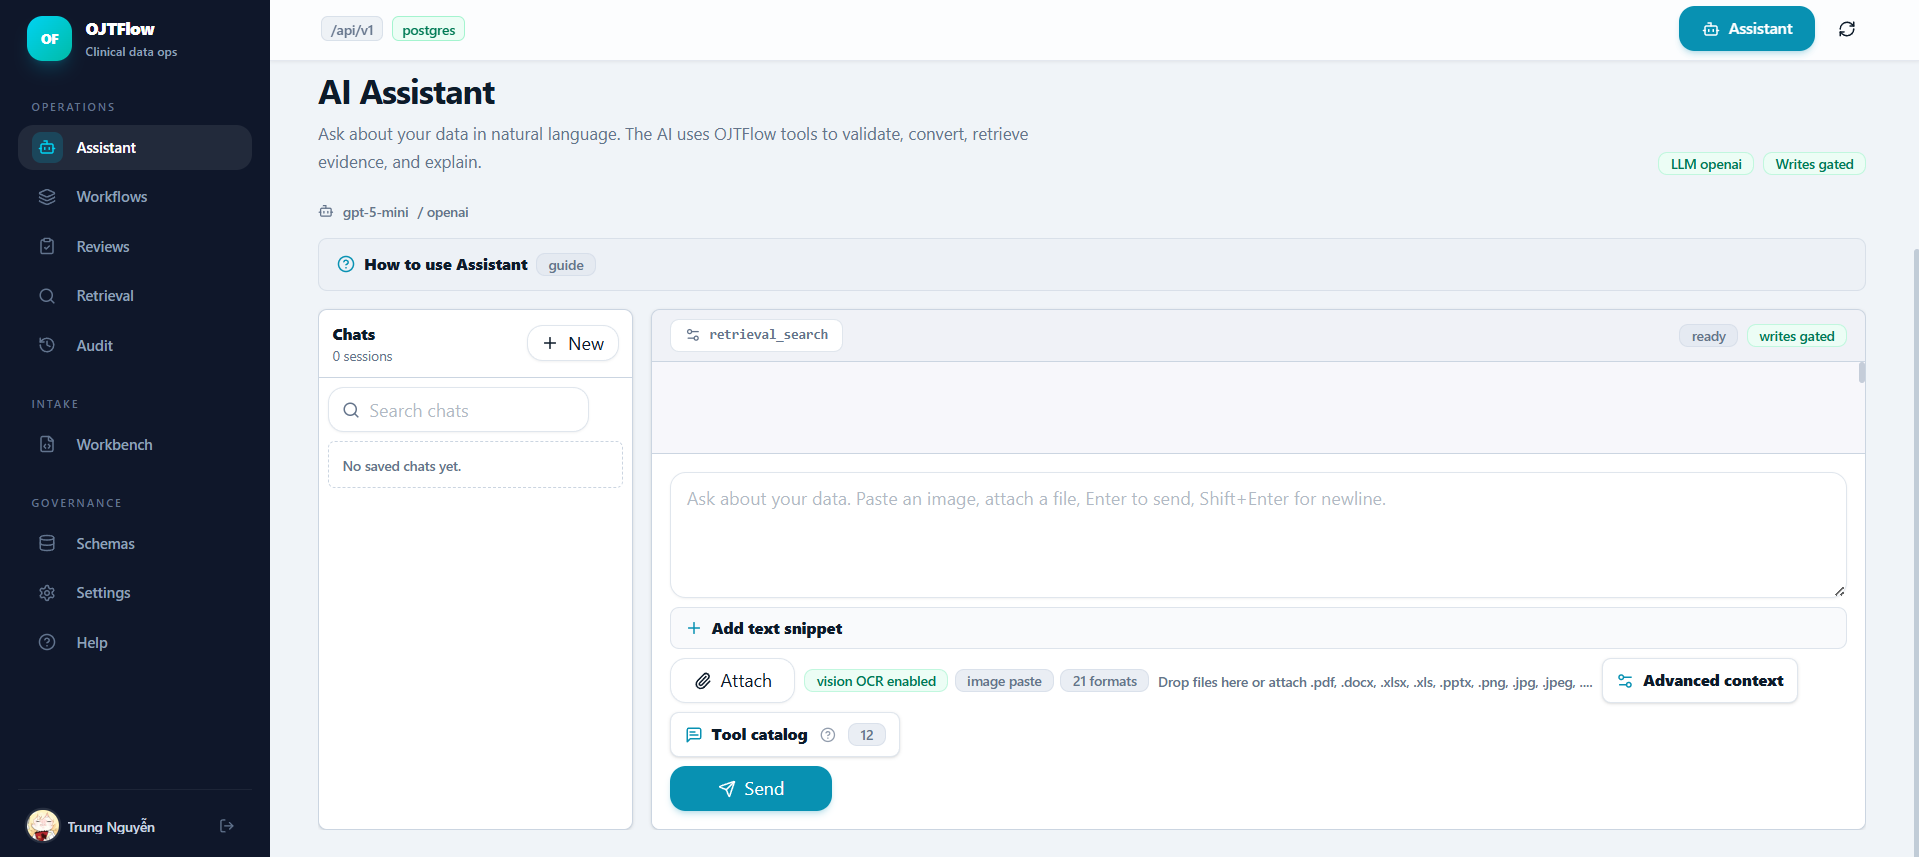
\includegraphics[width=13.2cm]{screenshots/main-assistant.png}
  };
\end{tikzpicture}

\vspace{5pt}
{\scriptsize\color{muted}RAG検索、OCRアップロード、ツールカタログ、書き込みゲート付き操作のデモUI。}
\end{frame}

% ═══════════════════════════════════════════════════════════════════════
% SLIDE 15: Thank You
% ═══════════════════════════════════════════════════════════════════════
{
\setbeamercolor{background canvas}{bg=dark}
\begin{frame}[plain]
  \vfill
  \begin{tikzpicture}[remember picture,overlay]
    \node[fill=primary, rounded corners=8pt, minimum size=36pt,
          anchor=north east] at ([xshift=-24pt,yshift=-20pt]current page.north east)
      {\large\bfseries\color{white}OJT};
  \end{tikzpicture}
  \begin{center}
    {\LARGE\bfseries\color{white}ありがとうございました}\\[12pt]
    {\normalsize\color{primary}基盤モデル + RAG + 永続KG + MCP + マルチエージェント}\\[5pt]
    {\small\color{muted}医療データガバナンス運用システム}\\[30pt]
    {\small\color{muted}ご質問は？\quad|\quad HuReDee-IoYou AI OJT}
  \end{center}
  \vfill
\end{frame}
}

\end{document}
